\graphicspath{{main/design/runtime/graphics/}}

\subsection{Analysis}

To select the most optimal environment to develop the software infrastructure upon, a series of benchmarking activities were carried out. These focused on evaluating the operating systems and hypervisors which could operate in a real-time environment. Comparing bare-metal Linux and Xen with Linux VMs should give a good method to estimate the specific latencies brough about by Xen.

\subsubsection{Test Suite}
There are several tools that can be used to analyse the real-time performance of an operating system. RT-Tests is a test suite that contains programs to test the various real-time Linux features.

The RT-Tests suite includes a cyclictest program. This is a simple yet effective program that can be used to estimate the real-time latencies in a system. It measures real-time jitter by creating a interrupt event at a specific time in the future and measuring the time delay between the requested wake-up and actual wake-up time. While this provides a good method for identifying operating system induced latency and jitter it does not isolate latencies induced by hardware or low-level firmware. At this stage it can be assumed that the selected development targets do not induce significant latencies.

% Stress-ng
Another tool that can be used during real-time testing is stress-ng (stress next generation) from \textcite{kingColinIanKingStressng2024}. This program can put artificial loads onto a Linux system. While sustained memory and CPU pressures are unlikely in a real application scenario it is important to ensure that the real-time characteristics of an OS do not significantly change.

\clearpage

\subsubsection{Previous Work}

% The paper results
\textcite{abeniUsingXenKVM2020} compiled a similar study into the real-time performance of open source hypervisors. Every hypervisor introduces some latencies into a virtual machine that can affect the correctness of the existing real-time analysis. They compared the performance of both KVM and Xen on various intel x86 processors.

The study found that the KVM hypervisor would be suitable for serving real-time workloads with worst-case latencies under $100\mu$s. This is applicable only when using RT kernels on both the guest and host. Likewise when using the Xen hypervisor the RT kernels on both the guest and host must also be used. Para-virtualised (PV) guests performed well but fully virtualised (HVM) guests did not, under $100\mu$s versus $1000000\mu$s.

% How it applies and differs from our tests
For the purpose of this project the real-time performance on an Arm64 target, the chosen development target, must be specifically analysed. It was reasonable to expect that the performance characteristics may be different between Arm64 and x86 due to the implementation of virtualisation extensions.

\clearpage

\subsubsection{Linux}

To set a baseline the real-time behaviour of Linux with the standard PREEMPT kernel was tested with different artificial loads in the system. Each test ran for exactly 1 hour collecting latency information at an interval of $100{\mu}s$.

Figure \autoref{fig:linux-i100-1h-allcores} displays that when not under load, the standard Linux kernel performs well in a real-time environment. However as soon as load was introduced into the system \autoref{fig:linux-i100-1h-allcores-sc4} and \autoref{fig:linux-i100-1h-allcores-sm4} the real-time performance was significantly worse.

\begin{figure}[ht]
    \centering
    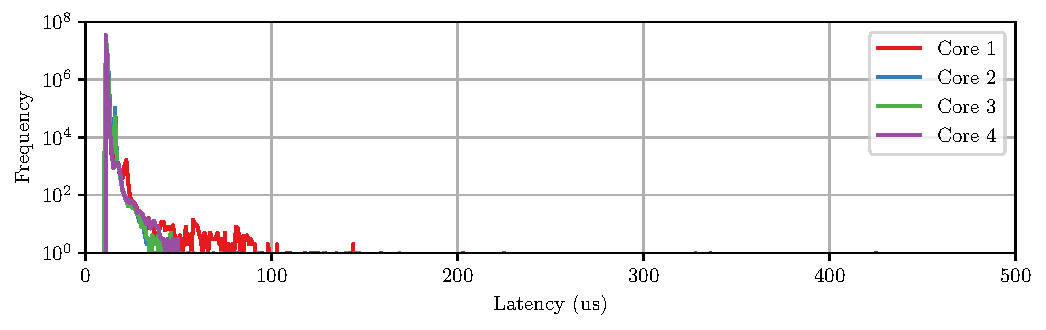
\includegraphics[width=\textwidth]{linux-i100-1h-allcores.pdf}
    \caption[Linux PREEMPT i100 cyclictest results (idle)]
    {Linux PREEMPT i100 cyclictest results (idle)}
    \label{fig:linux-i100-1h-allcores}

    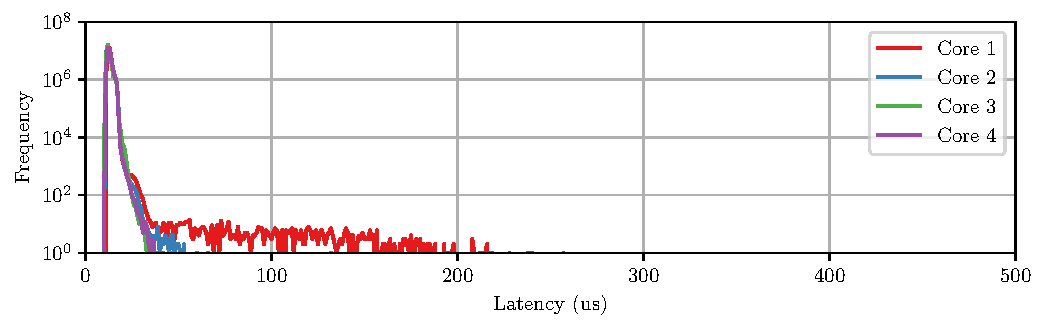
\includegraphics[width=\textwidth]{linux-i100-1h-allcores-sc4.pdf}
    \caption[Linux PREEMPT i100 cyclictest results (cpu load)]
    {Linux PREEMPT i100 cyclictest results (CPU load)}
    \label{fig:linux-i100-1h-allcores-sc4}

    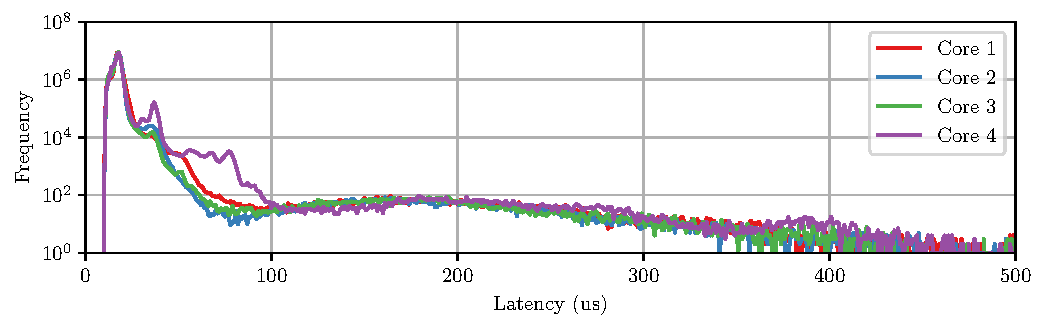
\includegraphics[width=\textwidth]{linux-i100-1h-allcores-sm4.pdf}
    \caption[Linux PREEMPT i100 cyclictest results (memory load)]
    {Linux PREEMPT i100 cyclictest results (memory load)}
    \label{fig:linux-i100-1h-allcores-sm4}
\end{figure}

\clearpage

The following tests in \autoref{fig:linux-rt-i100-1h-allcores}, \autoref{fig:linux-i100-1h-allcores-sc4} and \autoref{fig:linux-rt-i100-1h-allcores-sm4} all used the PREEMPT\_RT kernel. With the same test parameters the system maintained a good response latency even when under load.

\begin{figure}[ht]
    \centering
    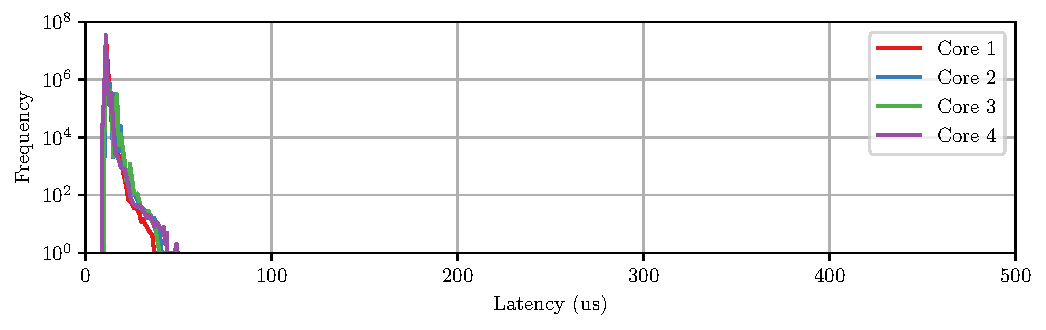
\includegraphics[width=\textwidth]{linux-rt-i100-1h-allcores.pdf}
    \caption[Linux PREEMPT\_RT i100 cyclictest results (idle)]
    {Linux PREEMPT\_RT i100 cyclictest results (idle)}
    \label{fig:linux-rt-i100-1h-allcores}

    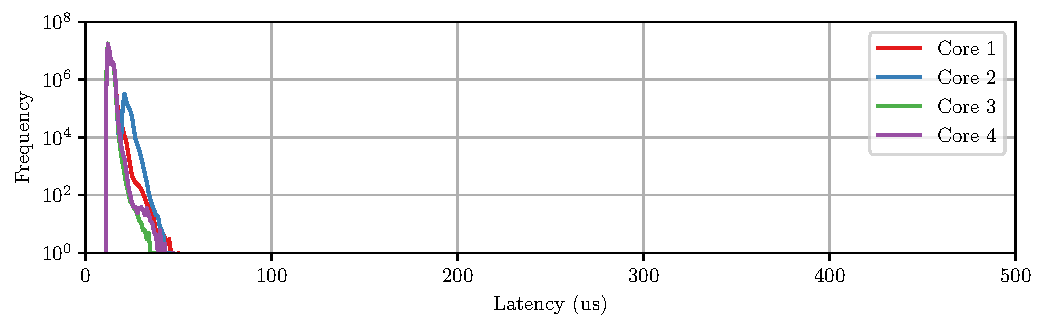
\includegraphics[width=\textwidth]{linux-rt-i100-1h-allcores-sc4.pdf}
    \caption[Linux PREEMPT\_RT i100 cyclictest results (cpu load)]
    {Linux PREEMPT\_RT i100 cyclictest results (cpu load)}
    \label{fig:linux-rt-i100-1h-allcores-sc4}

    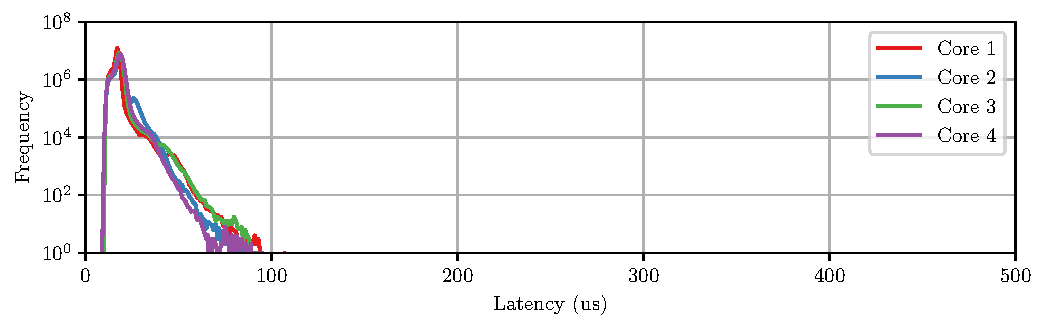
\includegraphics[width=\textwidth]{linux-rt-i100-1h-allcores-sm4.pdf}
    \caption[Linux PREEMPT\_RT i100 cyclictest results (memory load)]
    {Linux PREEMPT\_RT i100 cyclictest results (memory load)}
    \label{fig:linux-rt-i100-1h-allcores-sm4}
\end{figure}

\clearpage

\textbf{Evaluation}

The comparison between both kernels is shown in \autoref{fig:linux-vs-rt-linux-i100-1h-sc4} and \autoref{fig:linux-vs-rt-linux-i100-1h-sm4} displays that the real-time kernel patch works as expected.

Memory tests particularly strained the memory resources allocation processes of the kernel and affected the real time performance more than CPU load. This is because many parts of the Linux kernel resource allocation have indeterminate maximum latencies, as found in section \ref{sec:operatingSystems}.

% CPU LOAD - PREEMPT vs PREEMPT\_RT
\begin{figure}[ht]
    \centering
    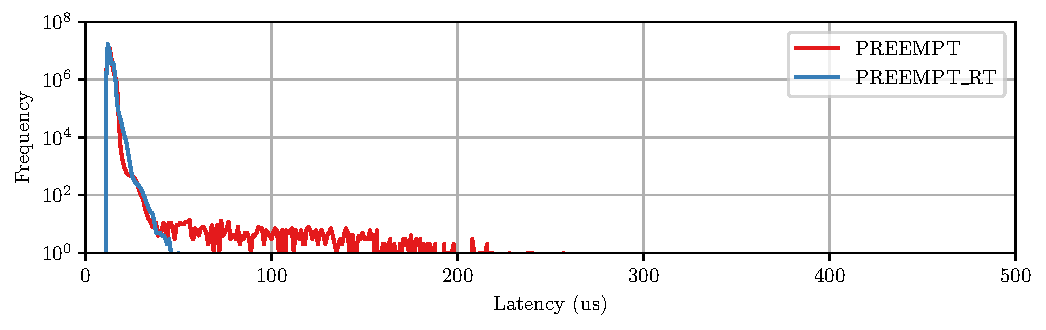
\includegraphics[width=\textwidth]{linux-vs-rt-linux-i100-1h-sc4.pdf}
    \caption[Linux PREEMPT vs PREEMPT\_RT i100 cyclictest results (cpu load)]
    {Linux PREEMPT vs PREEMPT\_RT i100 cyclictest results (cpu load)}
    \label{fig:linux-vs-rt-linux-i100-1h-sc4}
\end{figure}

% MEM LOAD - PREEMPT vs PREEMPT\_RT
\begin{figure}[ht]
    \centering
    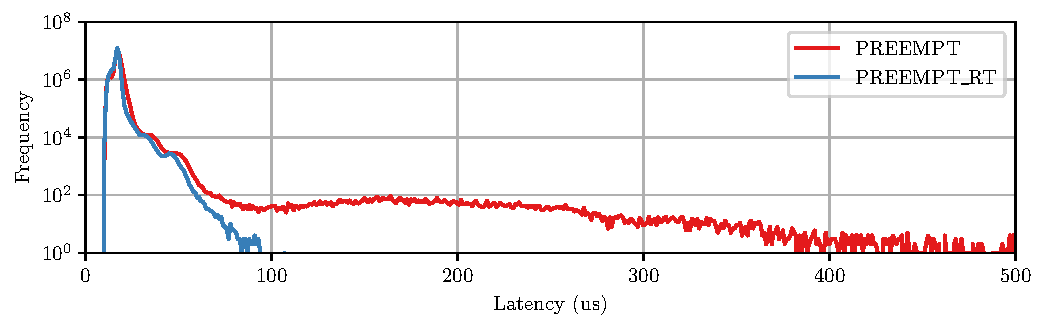
\includegraphics[width=\textwidth]{linux-vs-rt-linux-i100-1h-sm4.pdf}
    \caption[Linux PREEMPT vs PREEMPT\_RT i100 cyclictest results (memory load)]
    {Linux PREEMPT vs PREEMPT\_RT i100 cyclictest results (memory load)}
    \label{fig:linux-vs-rt-linux-i100-1h-sm4}
\end{figure}

\clearpage

\subsubsection{Xen Hypervisor}

After validating the Linux kernel's real-time response, the Xen hypervisor can be evaluated using Linux as both Dom0 and a DomU guest. To ensure that the Xen scheduler itself did not interfere with any results, all vCPUs were assigned on a one to one mapping of real CPUs using the 'null' scheduler. 

As shown in \autoref{fig:xen-rt-slop-i100-1h}, when Xen was evaluated using rt-tests at an interval of $100{\mu}s$ an almost even distribution of latencies is produced. This is very different to what was observed with bare-metal Linux.

\begin{figure}[ht]
    \centering
    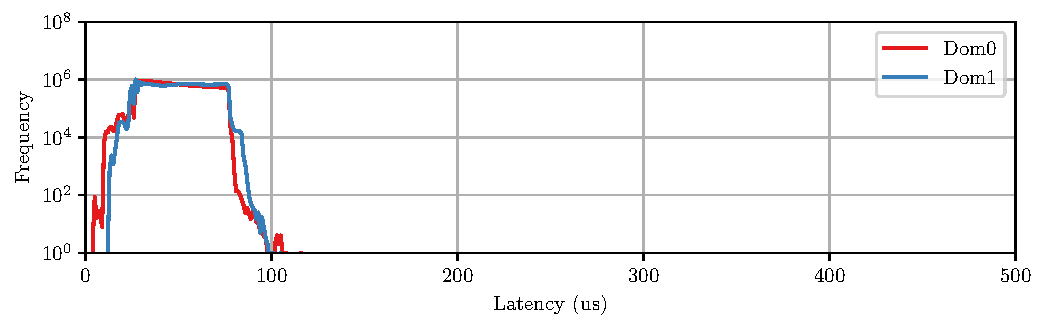
\includegraphics[width=\textwidth]{xen-rt-slop-i100-1h.pdf}
    \caption[Xen i100 cyclictest results (idle)]
    {Xen i100 cyclictest results (idle)}
    \label{fig:xen-rt-slop-i100-1h}
\end{figure}

In attempt to find the cause of the increased latencies, Xen was measured again at a range of intervals ($100{\mu}s$, $200{\mu}s$, $500{\mu}s$ and $1000{\mu}s$) in \autoref{fig:xen-rt-slop-i100-i1000-1h}. The even distribution affect is less noticeable on tests with larger intervals.

\begin{figure}[ht]
    \centering
    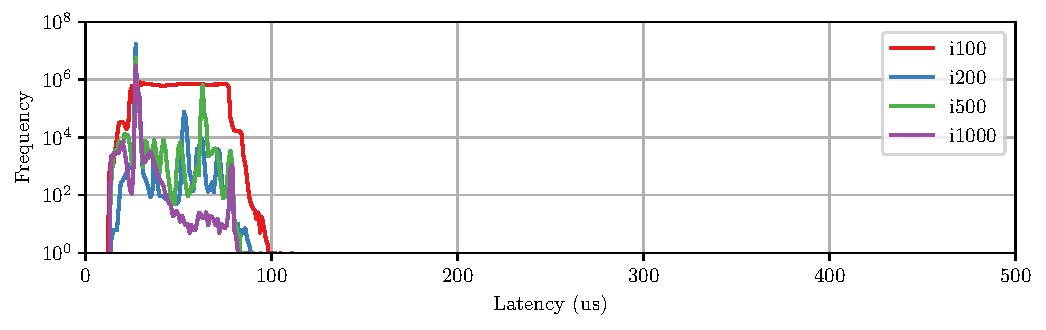
\includegraphics[width=\textwidth]{xen-rt-slop-i100-i1000-1h.pdf}
    \caption[Xen i100, i200, i500, i1000 cyclictest results (idle)]
    {Xen i100, i200, i500, i1000 cyclictest results (idle)}
    \label{fig:xen-rt-slop-i100-i1000-1h}
\end{figure}

This problem has connotations to the issues \textcite{abeniUsingXenKVM2020} experienced with timer resolutions negatively affecting latency evaluations. As cyclictest uses the local CPU timer to measure latencies it is important that it is at a high-enough resolution.

\clearpage

In a PVH virtualisation environment the CPU timers are often virtualized, hence they must be virtualised at high-enough resolution for cyclictest to use. By modifying the \verb|timer_slop| command line property in Xen to $1{\mu}s$ from $50{\mu}s$ the timer resolution was significantly increased. This resulted in much better performance metrics at intervals of $100{\mu}s$ in \autoref{fig:xen-rt-i100-i1000-1h}.

\begin{figure}[ht]
    \centering
    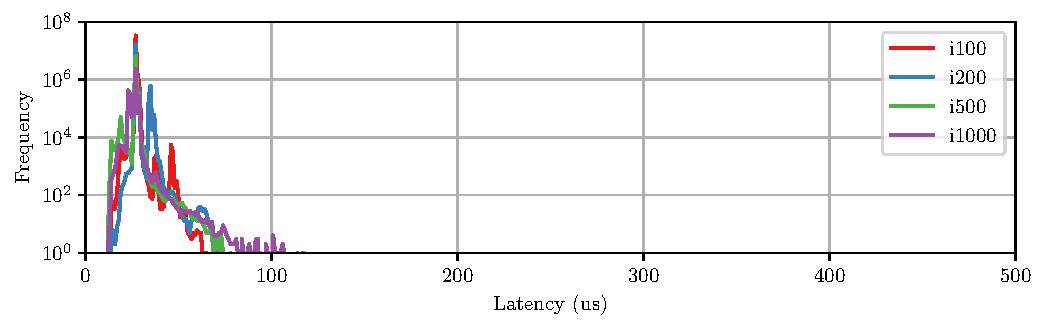
\includegraphics[width=\textwidth]{xen-rt-i100-i1000-1h.pdf}
    \caption[Xen timer adjustment i100, i200, i500, i1000 cyclictest results (idle)]
    {Xen timer adjustment i100, i200, i500, i1000 cyclictest results (idle)}
    \label{fig:xen-rt-i100-i1000-1h}
\end{figure}

To confirm the real-time performance, Xen was also tested with artificial CPU loads in Dom0 and DomU. \autoref{fig:xen-rt-i100-i1000-1h-sc1} shows that there is negligible differences as compared to without load. 

\begin{figure}[ht]
    \centering
    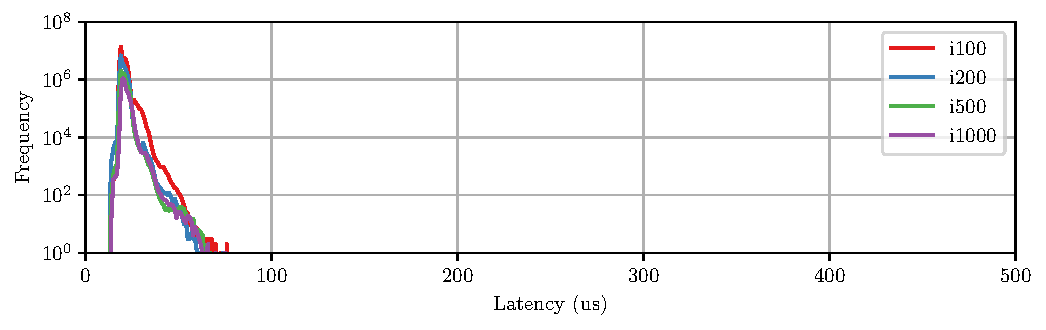
\includegraphics[width=\textwidth]{xen-rt-i100-i1000-1h-sc1.pdf}
    \caption[Xen timer adjustment i100, i200, i500, i1000 cyclictest results (cpu load)]
    {Xen timer adjustment i100, i200, i500, i1000 cyclictest results (cpu load)}
    \label{fig:xen-rt-i100-i1000-1h-sc1}
\end{figure}


\textbf{Evaluation}

Xen approximately doubled the interrupt latency measured as compared to bare-metal Linux. This is not ideal, but Xen could still be used in a soft real-time application if the latencies were accounted for. Before deploying Xen in a real-time environment, additional tests should evaluate the multi-core interference across multiple guest virtual machines.
